\documentclass[a4paper,12pt]{article}
   % Packages and definitions:
   % {
      \usepackage{float}
      \usepackage[english]{babel}
      \usepackage[utf8]{inputenc}
      \usepackage{amsmath}
      \usepackage{amssymb}
      \usepackage{color}
      \usepackage{subcaption}
      \usepackage{booktabs}
      \usepackage{tikz}
      \usepackage{multirow}
      \usetikzlibrary{decorations.pathreplacing}
      \usepackage{graphicx,epstopdf}
      \usepackage{cleveref}
      \usepackage{collcell} % loads array
      \usepackage{listings}
      \usepackage{algorithm}
      \usepackage{algpseudocode}
      \usepackage{epstopdf}
      \newcolumntype{m}{>{$} r <{$}}
      \newcolumntype{u}{>{$[\collectcell\si} l <{\endcollectcell]$}}
      \newcommand{\approxtext}[1]{\ensuremath{\stackrel{\text{#1}}{=}}}
      \newcommand{\matr}[1]{\mathbf{#1}}
      \newcommand{\partt}[2]{\ensuremath{\dfrac{\d {#1}}{\partial {#2}}}}
      \renewcommand{\d}[1]{\ensuremath{\operatorname{d}\!{#1}}} % non-italized differentials
      \newcommand{\h}[0]{\ensuremath{\hbar}} % hbar
      \newcommand{\qed}[0]{\ensuremath{\tag*{$\square$}}} % QED square
      \def\changemargin#1#2{\list{}{\rightmargin#2\leftmargin#1}\item[]}
      \let\endchangemargin=\endlist 
      \usepackage{amsthm}
      \theoremstyle{plain}
      \newtheorem{thm}{theorem} % reset theorem numbering for each chapter
      \theoremstyle{definition}
      \newtheorem{defn}[thm]{definition} % definition numbers are dependent on theorem numbers
      \newtheorem{exmp}[thm]{example} % same for example numbers
      \bibliographystyle{natbib}
      \renewcommand{\theequation}{\thesection.\arabic{equation}}
      \newcommand{\ts}{\textsuperscript} 

      \definecolor{dkgreen}{rgb}{0,0.6,0}
      \definecolor{gray}{rgb}{0.5,0.5,0.5}
      \definecolor{mauve}{rgb}{0.58,0,0.82}

      \lstset{frame=tb,
        language=Java,
        aboveskip=3mm,
        belowskip=3mm,
        showstringspaces=false,
        columns=flexible,
        basicstyle={\small\ttfamily},
        numbers=none,
        numberstyle=\tiny\color{gray},
        keywordstyle=\color{blue},
        commentstyle=\color{dkgreen},
        stringstyle=\color{mauve},
        breaklines=true,
        breakatwhitespace=true,
        tabsize=3
      }
% }
\title
{
	\textbf
	{
      Single and Multi-layer perceptrons for classifications and predictions of
      time series
   }
}

\author{Henrik Åhl\\}
\date{\today}

\begin{document}
\begin{titlepage}
	
   \maketitle 
	\begin{center}
		\phantom{a}
		{Department of Astronomy and Theoretical Physics, Lund University}
		\\[2cm]
		{Project supervised by Mattias Ohlsson}
		\vfill
		\includegraphics[height=4cm]{logocLUeng.pdf}
	\end{center}
	\thispagestyle{empty} % do not count pages just yet

\end{titlepage}

\vspace{5cm}
\noindent\textit{And this all works extremely well. Or, at least it works.}\\ --- Mattias Ohlsson, 2015
\newpage

\section{Introduction}
   Neural networks can be used for a wide range of purposes, ranging from
   function approximation to identifying patterns in images. Although the
   networks themselves can be constructed to be however complicated the creator
   wishes, relatively simple networks can be shown to be able to solve
   complicated tasks. Especially single-layer perceptrons, as are the main study in
   this report, are able to perform surprisingly complex tasks.

\section{Problems}
	\setcounter{equation}{0}
   \subsection{Competitive networks for clustering}
   % 1
      In using the VQ model for classification, it is apparent that the method
      indeed is able to correctly find the different class centers in many
      cases. In the few occurences where it is not the case, the ambiguity stems
      from outputs getting stuck between two classes, with equal tendencies to
      shift towards either one. It is however possible that these happenings
      often will eventually vanish given more computed epochs, due to the
      inherent flucutations of the system.

      \begin{figure}[H]
         \centering
         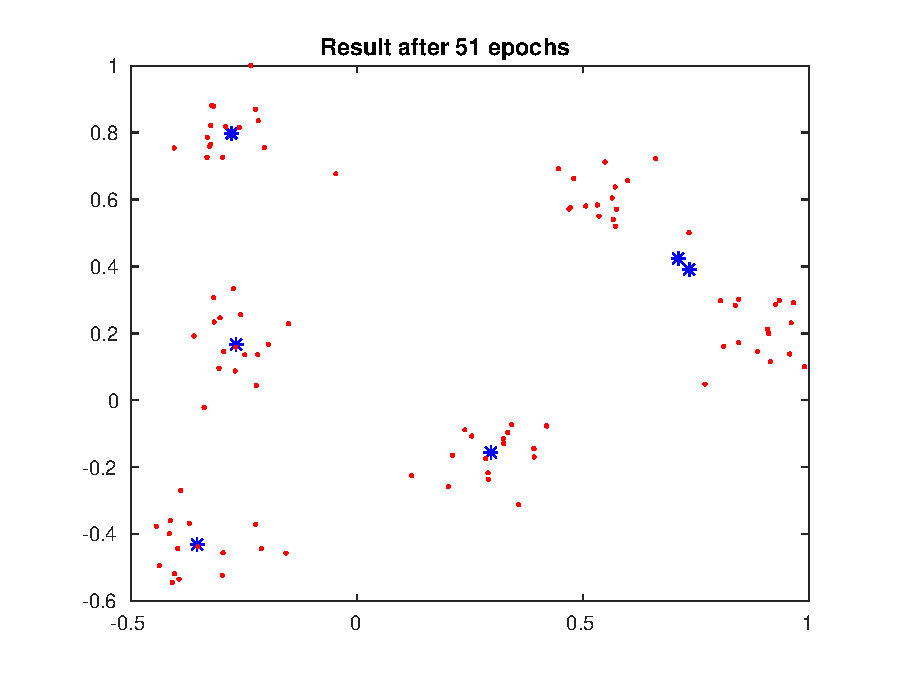
\includegraphics[scale=.6]{1}
         \caption{Clustering result with the VQ algorithm. Note the ambiguous
         nodes in the top right corner. }
         \label{fig:1}
      \end{figure}
   
   % 2
      When the default settings are changed, so that the bias learning rate is
      set to zero, so called dead neurons appear -- neurons that get stuck far
      away from clusters due to the algorithm favoring the update of neurons
      close to data clusters. It is also apparent that the value of the bias
      learning rate is significantly lower than the ordinary one, as the neurons
      otherwise become extremely likely to not move at all, resulting in a
      cluster of its own of dead neurons.

   % 3
      Furthermore, when superfluous neurons are introduced, they severely affect
      the performance of the VQ method. As there in that case tends to be
      several ``winning neurons'', the neurons counteract each other, resulting
      in them instead merely encircling or approaching the very cluster centers they 
      are meant to find. It is also the case that more neurons give rise to heavier
      interference, and thus also worse overall performance.
      
      \begin{figure}[H]
         \centering
         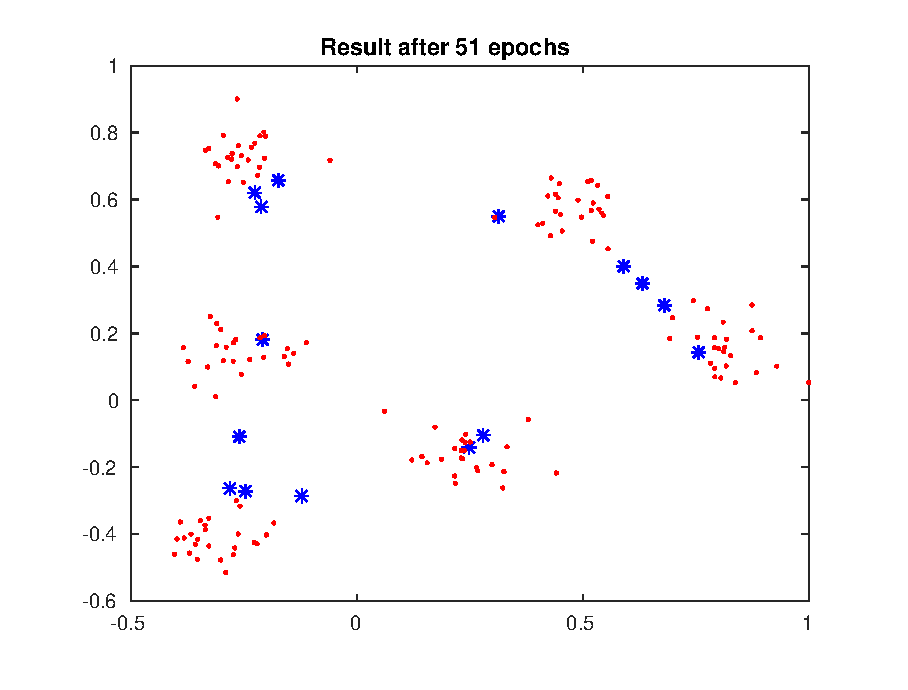
\includegraphics[scale=.6]{3}
         \caption{Clustering result with the VQ algorithm and superfluous
         neurons. Especially consider the upper right corner, which like in the
         previous case attracts ambiguous neurons.}
         \label{fig:3}
      \end{figure}

      \subsection{ORL face data}
   % 4 & 5
      Interestingly enough, the competitive network manages to group different
      faces into categories fairly adequately; in almost all 80 cases, the
      network manages to find the corresponding two pictures of the same person.
      Moreso, with 6 output nodes used, the network groups a significant amount of the
      occuring faces with similar attributes into the same categories. The most
      defining trait with determines grouping seems to be the skin tone, or the
      brightness of the photograph, as it is highly related to the color of a majority of
      the pixels in every picture. However, also people with other similarities are
      frequently grouped together, such as people with glasses or people with a
      similar haircut, which ought to be because similarly colored pixels appear
      in similar places, which causes the network to identify the shared
      attribute. Also when performed several times, the network tends to give
      similar results, grouping people into roughly the same categories as
      before. 

      There does however appear to be a significant bias towards beloning to the
      first groups (i.e. laying close to node 1 etc.), which suggests that some
      data points again get stuck due to conflicting algorithmic interests.

      \begin{figure}[H]
         \centering
         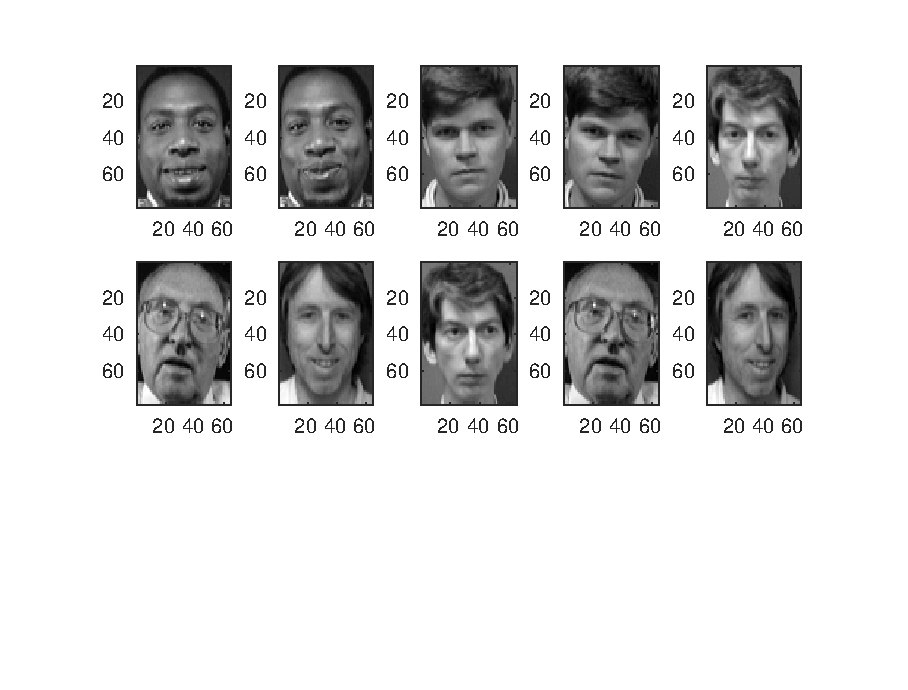
\includegraphics[scale=.8,trim=0 4cm 0 0]{45}
         \caption{Cluster category produced by the VQ algorithm. Note the
         similarities in the overall tone of the images.}
         \label{fig:45}
      \end{figure}

      
      When further performing the analysis on as many as 40 nodes, i.e. as many
      nodes as there are different people, and iterating over many epochs, the
      network is fairly able to group together the corresponding two pictures of
      two people, being able to do so correctly in as many as $10/40$ cases,
      where several of the remaining fraction still contains correct matchups,
      though with 3 or more individuals beloninging to that group. Again,
      however, there is a strong bias towards the lowest labeled nodes in the network.
   
   %  4-5 avg
      As the cluster centers can be identified as the ``average'' person within
      a cluster, it can be amusing to witness the result, here exemplified in~\cref{fig:45avg}. 
      As to be expected, the average individual corresponds to an
      overlap between the images belonging to that specific cluster. 
      
      \begin{figure}[H]
         \centering
         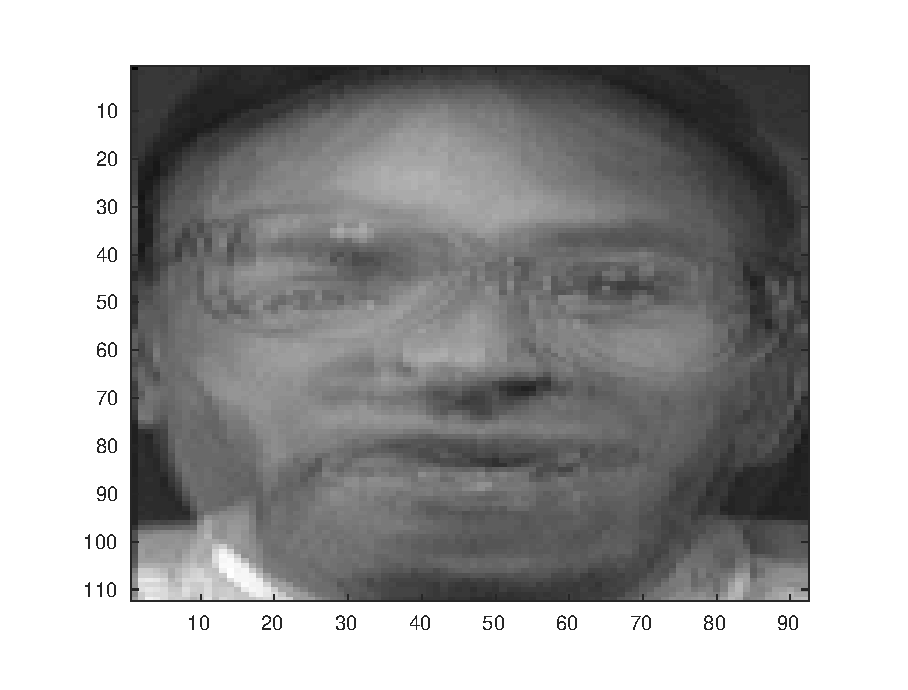
\includegraphics[scale=.6]{45avg}
         \caption{Example image corresponding to the weight vector defining
         a cluster center.}
         \label{fig:45avg}
      \end{figure}

      \subsection{SOFM}

   % 6
      With the SOFM method, clusters in the data set tend to attract a concentration of
      output nodes in one or two dimensions. The higher the variance between
      data points, the further away their corresponding nodes will appear in
      weight space. These two attributes of the SOFM algorithm can easily be
      seen in \cref{fig:6}.
      
      \begin{figure}[H]
         \centering
         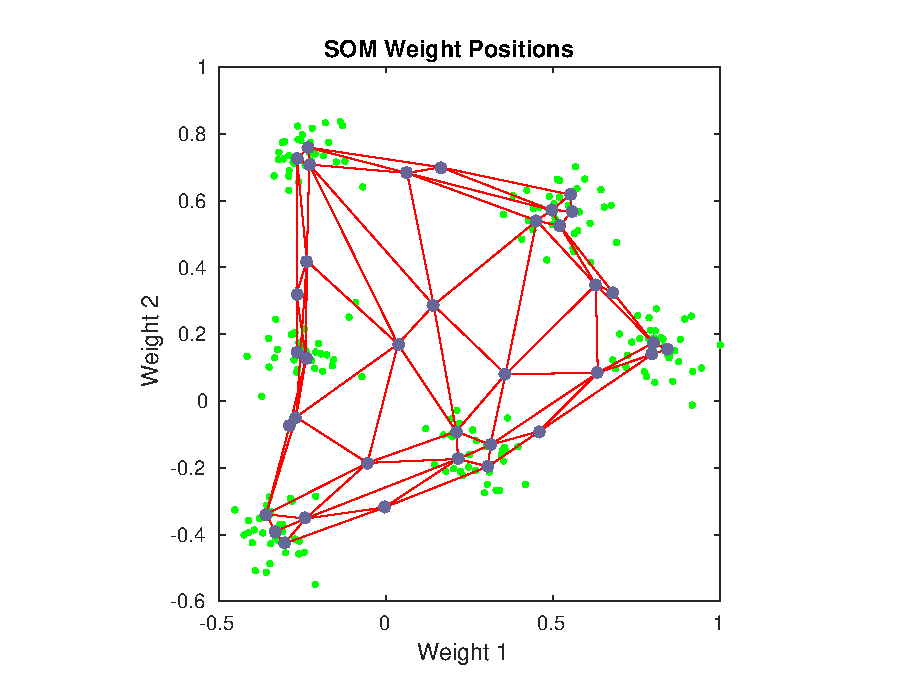
\includegraphics[scale=.6]{6}
         \caption{Weight positions for the SOFM algorithm. Clusters of data tend
         to attract clusters of nodes.}
         \label{fig:6}
      \end{figure}

% 7
      From a quick analysis of the SOFM performance in grouping faces together,
      under an image size reduction to $50~\%$,
      it seems to be, from a subjective viewpoint, worse than the simple clustering
      method. Although it indeed manages to group corresponding face pairs in
      the same category to roughly the same performance as in the clustering
      case, there cannot be said to be any clear similarities between pairs. In
      the clustering case, for example, people with glasses were likely to end
      up in the same category, which cannot be said to be the effect of the SOFM. 

      Notably enough however, when the image reduction is skipped completely,
      the SOFM net shows significant improvements, even passing the performance
      of the VQ net. The grouping in this case differs from the VQ net in that
      it seems to find similar features that the former could not, such as
      expressions (smiles etc.) and face shapes -- at least to a higher degree.
      Also the previously occuring group of men with beards and glasses again
      appear, as shown in~\cref{fig:7_beardandglasses}, showing that image
      reduction does affect the performance of the network.
      
      \begin{figure}[H]
         \centering
         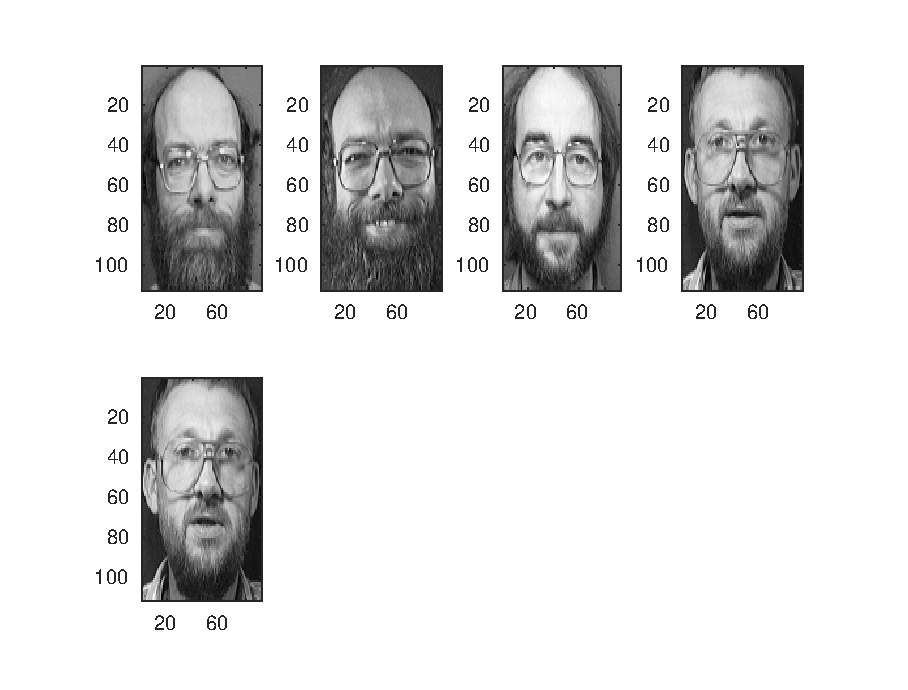
\includegraphics[scale=.6]{7_beardandglasses}
         \caption{Cluster produced of men with similar facial attributes. Note
         here that the skin tone is not as defining of a factor as in previous
         cases.}
         \label{fig:7_beardandglasses}
      \end{figure}

   % 8
      The distance between output nodes also indeed seems to be related to the
      features of the images. As in the previous case, the most defining
      attribute seems to be the overall brightness of the image. In particular in
      the comparision between \cref{fig:8_dark} and \cref{fig:8_light} this behaviour 
      of the network can be seen, as the two clusters
      correspond to points far from each other in weight space. 
      
      \begin{figure}[H]
         \vspace*{1cm}
         \hspace*{-2cm}
         \centering
         \begin{minipage}[t]{.6\textwidth}		
            \vspace{0pt}
            \centering
            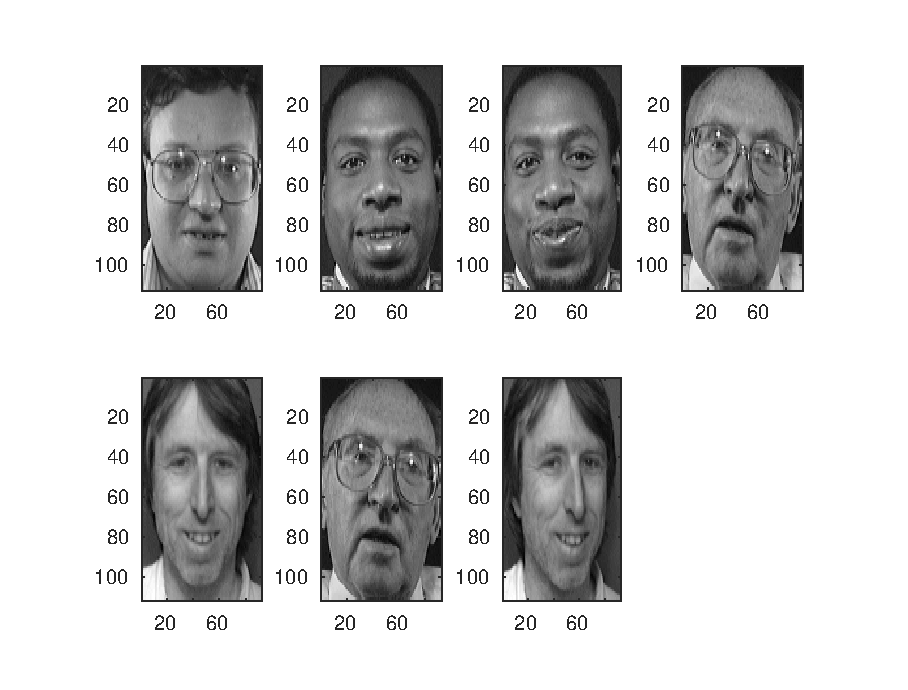
\includegraphics[scale=.6]{8_distancedark}
            \caption{Dark-face category.}
            \label{fig:8_dark}
         \end{minipage}~\hspace*{1em}
         \begin{minipage}[t]{.6\textwidth}		
            \vspace{0pt}
            \centering
            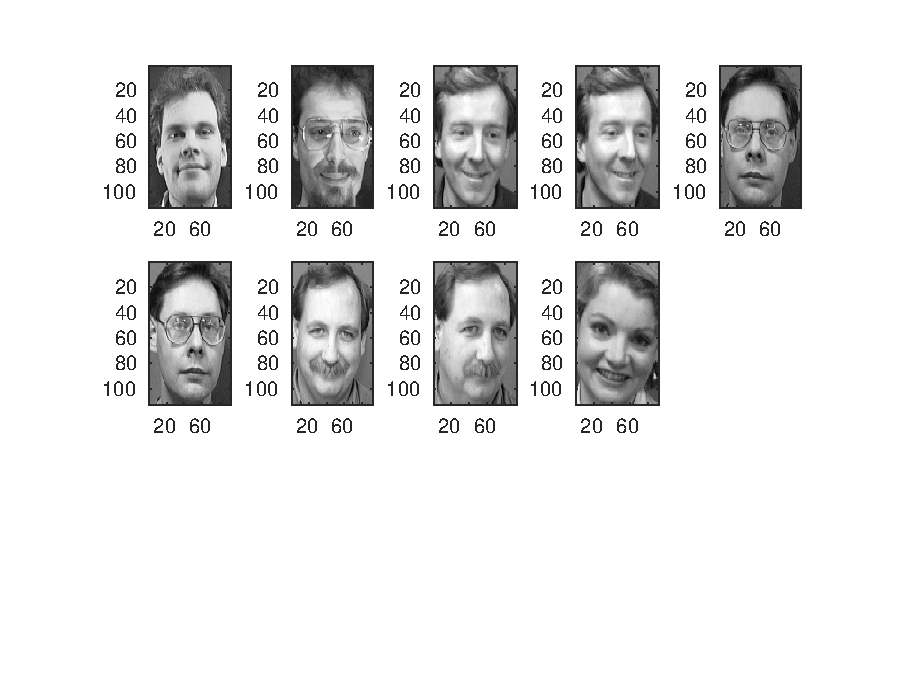
\includegraphics[scale=.6, trim=1cm 0 0 0]{8_distancelight}
            \caption{Light-face category.}
            \label{fig:8_light}
         \end{minipage}
      \end{figure}

      \subsection{LVQ} 
   % 9
      It seems clear from the analysis that at least six nodes are required to
      somewhat sufficiently classify the data points. This ought to be because
      of the need to define two areas -- one related to class 1, the
      other to class 2. The corresponding decision boundary is then made up by
      weighting of the nodes determining ``cluster centers''. This is shown in 
      \cref{fig:9}, where the nodes are seen distributed throughout the data
      points in order to delimit the two classes, in
      effect defining a decision boundary with a closed geometry. 
      
      With a slightly lower learning rate than the default one, the best network 
      trained managed to classify $92~\%$ of the data points correctly, roughly on par with the
      15-node, two-layer network result in homework assignment 1.  
      
      \begin{figure}[H]
         \centering
         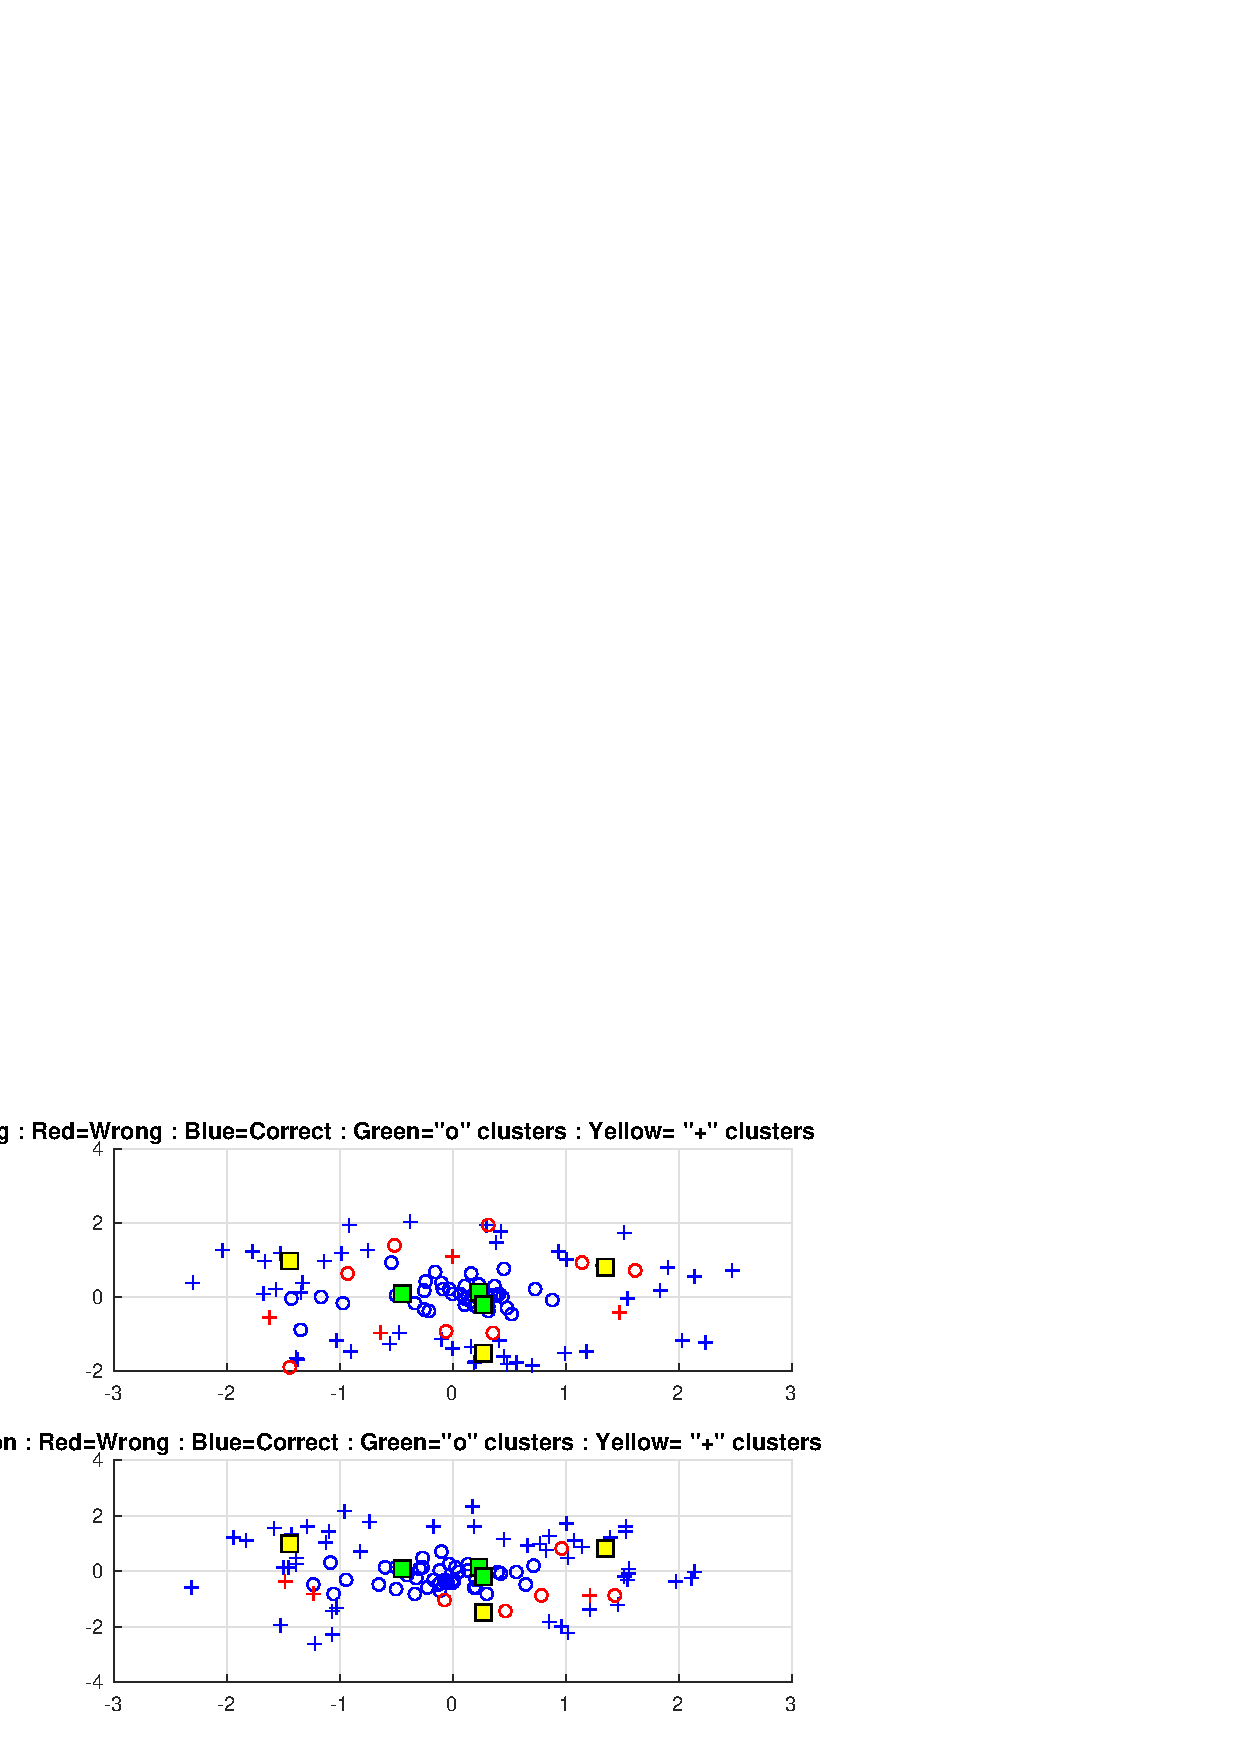
\includegraphics[scale=.6]{9}
         \caption{Visualization of training and validation performance. The
         cluster centers belonging to the two classes respectivelly are spread
      out in order to properly weight the classification boundary in place.}
         \label{fig:9}
      \end{figure}

   \subsection{Time-Delay Networks}
   % 10
      Using an Elman net with one delay feedback into the loop, it can be seen
      by using an alternating number of neurons, that the ability of the net to
      predict time series quickly deteriorates the more nodes there are. For
      four and five hidden nodes, the network simply crashes completely, not being able to
      predict anything to a satisfying degree. Instead, for two and three hidden
      nodes, the network performs comparatively equally ($NMSE \sim 0.13$), producing a valid
      prediction of the time series. For a network with one hidden node, the
      output is on average slightly worse ($NMSE \sim 0.24$), mostly due to a slight shift in time, suggesting
      that the network indeed does a viable prediction, but is not able to align it
      phase-wise with actual data. This one-node Elman net performs roughly as
      well as the earlier sunspot predictors used in homework assignment one,
      which had a $NMSE$ on about the same level.
      
      \begin{figure}[H]
         \vspace*{1cm}
         \hspace*{-2cm}
         \centering
         \begin{minipage}[t]{.6\textwidth}		
            \vspace{0pt}
            \centering
            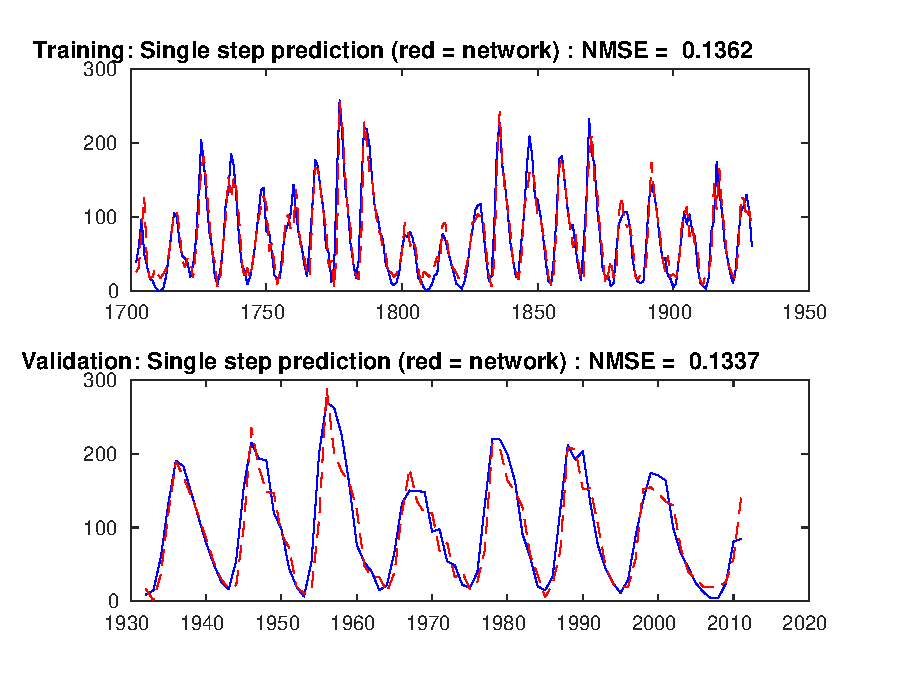
\includegraphics[scale=.6]{10_2_nodes}
            \caption{Elman network performance with two hidden nodes.}
            \label{fig:10_2}
         \end{minipage}~\hspace*{1em}
         \begin{minipage}[t]{.6\textwidth}		
            \vspace{0pt}
            \centering
            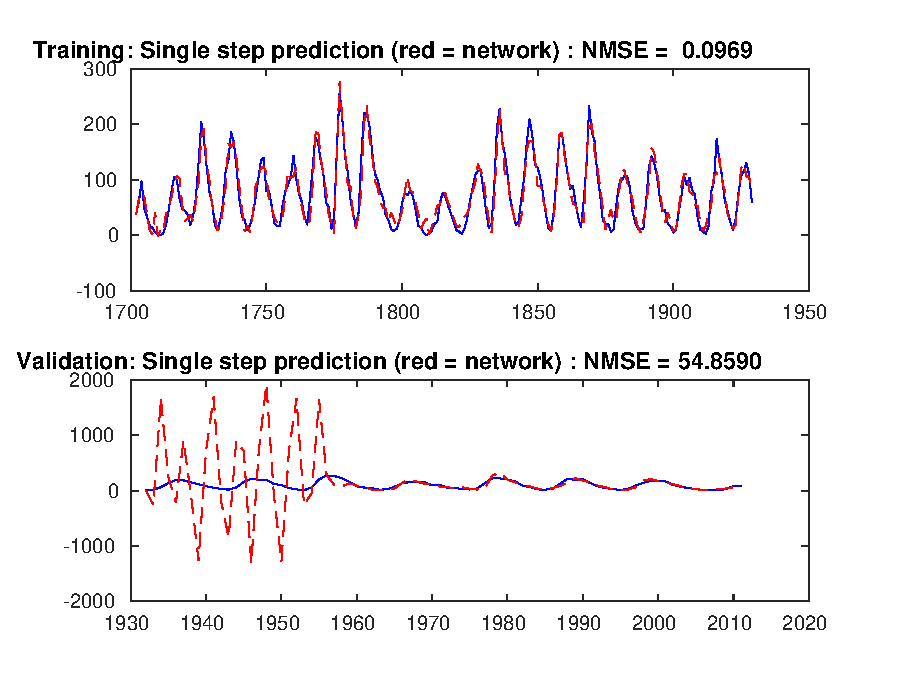
\includegraphics[scale=.6, trim=1cm 0 0 0]{10_5_nodes}
            \caption{Elman network performance with five hidden nodes. Extremely
            bad prediction of the time series although the training performance
            is better than the two node net.}
            \label{fig:10_5}
         \end{minipage}
      \end{figure}
   
   % 11
      Interestingly enough, from the analysis, the optimal time delay appears to
      be the one where the previous value is evaluated, i.e. a time delay of
      one. Contrary to what was achieved in assignment one then, the most
      determining previous value for the Elman net is the one occuring at
      $t' = t-1$, whereas we in the earlier assignment saw that a set with circa
      four of the preceding twelve outputs were the best at predicting the
      sunspot time series. (At least for me.) 

   \subsection{Hopfield Networks}
   
   % 12
      It can be shown that 0.138 patterns can be stored for each node, as done
      by Hertz et al 1991~\cite{hertz}. Using this rule of thumb and the fact
      that our images are represented by $7 \times 5$ nodes, we see that we can
      theoretically store at most 6 complete (random) patterns in our network.
      We must however realize that our patterns are not fully random, but
      correlated in appearance; consider for example the similarities between
      the letters $D$ and $E$ in low resolution. Consequently, all of our letters will
      not be stable, as we can most notably see in \cref{fig:12_eandb}, where the stored letter
      $E$ converges towards the representation of a $B$, with letters
      $A$--$E$ stored in the network.
      
      \begin{figure}[H]
         \centering
         \includegraphics[scale=.6]{12_eandb}
         \caption{Convergence for the letter $E$, which classifies as a
         $B$ after a few iterations.}
         \label{fig:12_eandb}
      \end{figure}

      Since the images are so compressed, even slight distortions will greatly
      affect the retrieval ability of the network. Although the similarities
      between the letters $A$ and $B$ are few, the letter $A$ will occasionally
      converge towards a $B$ even with as low of a distortion probability as
      0.1. Also the fact that inverted patterns are minima in the effective
      energy landscape is illustrated in \cref{fig:12_distortion}, as the
      $B$ is inverted relative to the stored letter. 
      
      In effect then, if the stored patters share similarities, the
      stability of patters certainly cannot be guaranteed, whereas if the images
      are also distorted, the retrieval rate is even further decreased.
      
      \begin{figure}[H]
         \centering
         \includegraphics[scale=.6]{12_distortion}
         \caption{Convergence for the distorted letter $A$ ($p=0.1$), which
            classifies as an inverted(!)
            $B$ after a few iterations.}
         \label{fig:12_distortion}
      \end{figure}

   % 13
      When ten letters are stored in the network, the limitations become even
      more apparent as there even without distortions will be huge
      instabilities, resulting in many spurious states. In fact, the only
      letters not converging towards spurious states, even without distortion, are the
      letters $I$ and $J$, where $J$ nontheless converges towards the stable $I$. 
      All in all then, $9/10$ stored patterns will in effect be unstable. Notably, the 
      letters $B, E$ and $F$ all converge towards the same spurious
      state, as do the letters $C, D$ and $G$. 

   % 14
      In the Matlab model however, all stored letters are stable. However, as
      with the original model, distorted patters are likely to end up in
      spurious states, even with low probabilities ($p = 0.1$) of flipping pixels. Out
      of all the ten letters, five are on average stable. 
      



%      \begin{figure}[H]
%         \centering
%         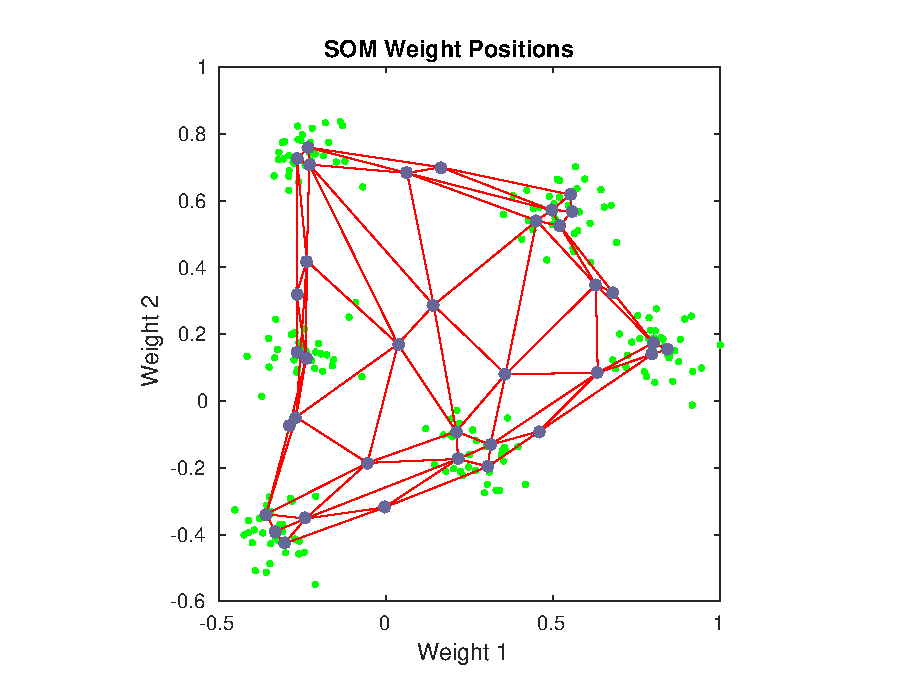
\includegraphics[scale=.6]{6}
%         \label{fig:6}
%         \caption{Graphical results of the training performance for the synthetic
%         data set. The linear function shows the decision boundary produced by the
%         neural network.}
%      \end{figure}

      
 %     \begin{figure}[H]
 %        \centering
 %        \includegraphics[scale=.6]{8_data}
 %        \label{fig:8_data}
 %        \caption{Depiction of the problematic in trying to discern the two
 %        classes from each other. The graph itself shows the validation performance of a
 %        15 node network.}
 %     \end{figure}

%      \begin{figure}[H]
%         \vspace*{1cm}
%         \hspace*{-2cm}
%         \centering
%         \begin{minipage}[t]{.6\textwidth}		
%            \vspace{0pt}
%            \centering
%            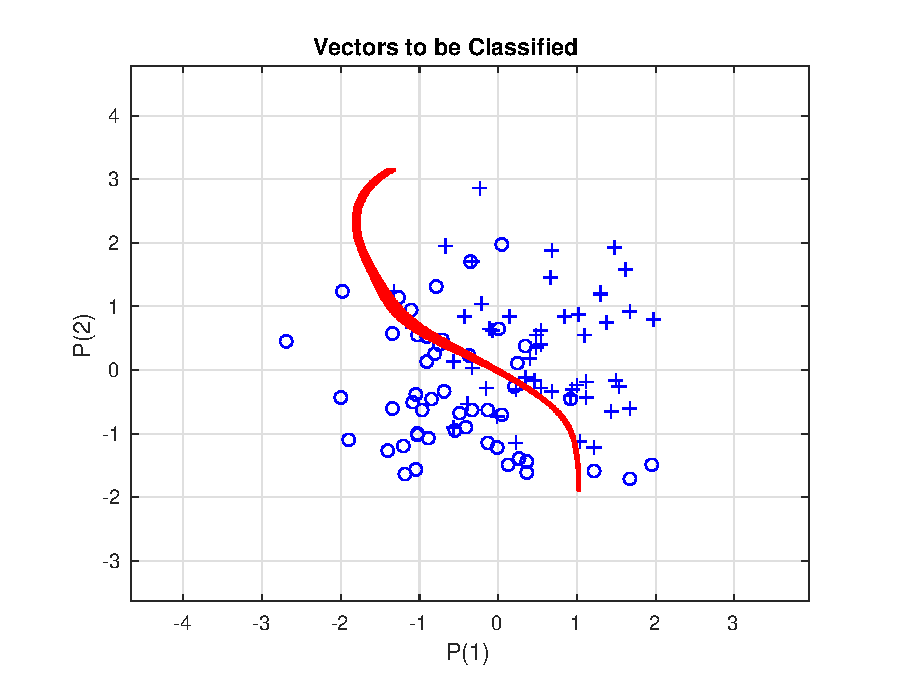
\includegraphics[scale=.6]{8_12_nodes}
%            \label{fig:8_12_nodes}
%            \caption{Classification output for synthetic data set 1, with 12
%            hidden nodes.}
%         \end{minipage}~\hspace*{1em}
%         \begin{minipage}[t]{.6\textwidth}		
%            \vspace{0pt}
%            \centering
%            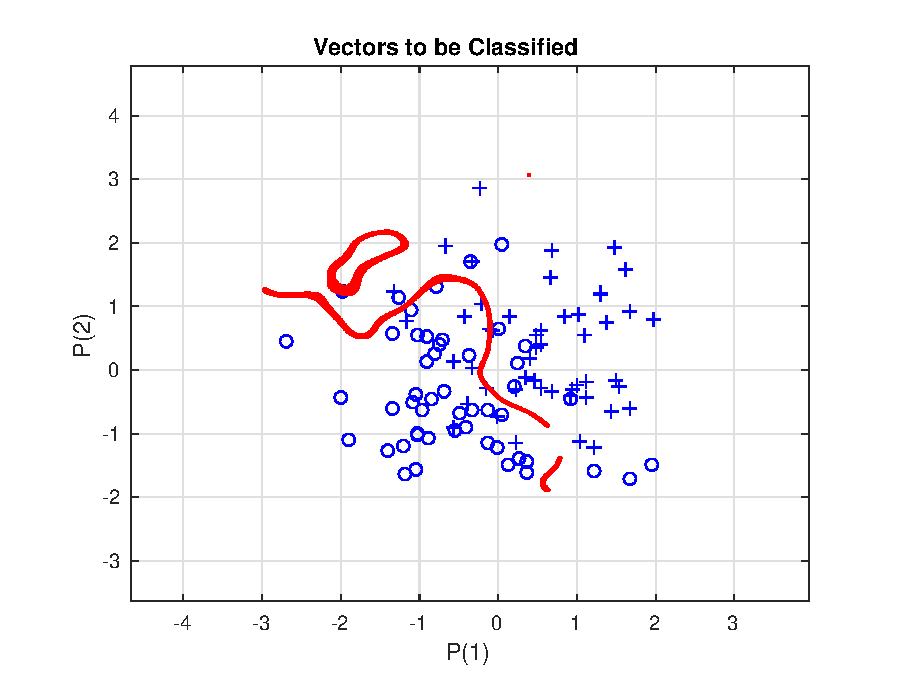
\includegraphics[scale=.6]{8_100_nodes}
%            \label{fig:8_100_nodes}
%            \caption{Classification output for synthetic data set 1, with 100
%            hidden nodes. Note that there are vague signs of overtraining relative to
%            fig.~3.}
%         \end{minipage}
%      \end{figure}
      
%      \begin{figure}[H]
%        \centering
%         \resizebox{.7\textwidth}{!}{\input{7.tex}}
%         \caption{Training versus validation performance (fraction of correct
%         classifications) on synthetic data set 1. Note that the validation
%         performance is consistently lower than the training one.}
%         \label{fig:7_and_8_comp}            
%      \end{figure}
      
      
%      \begin{figure}[H]
%         \centering
%         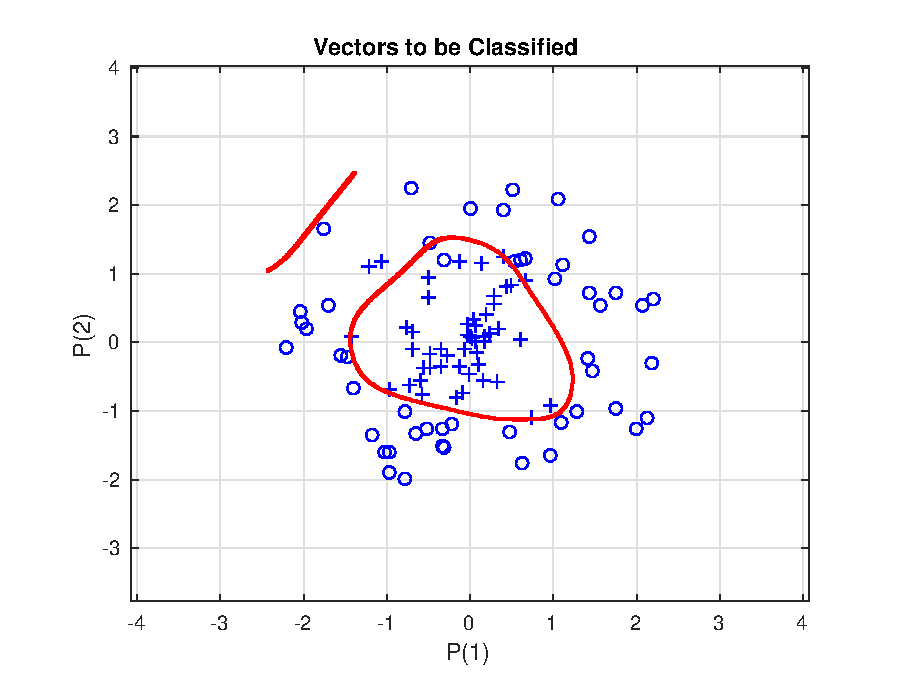
\includegraphics[scale=.6]{9_15_nodes}
%         \label{fig:9_data}
%         \caption{Training sample of synthetic data set 3. Graph shows training classification for a 15 node
%      network.}
%      \end{figure}
   
   \section{Concluding remarks}

   \begin{thebibliography}{99}
   \bibitem{lecnotes}
     Mattias Ohlsson,
     \emph{Lecture notes, Artificial Neural Networks},
     Department of Astronomy and Theoretical Physics,
     Lund University,
     2015.
   \bibitem{excnotes}
     Mattias Ohlsson,
     \emph{Exercise 2: Self-Organization and Feedback Networks},
     Department of Astronomy and Theoretical Physics,
     Lund University,
     2015.
   \bibitem{hertz}
      Hertz, J., Krogh, A., and Palmer, R.G.;
      \emph{Introduction to the theory of neural computation}, 
      Redwood City, CA: 
      Addison-Wesley,
      1991. 

\end{thebibliography}
%\newpage
%\appendix
%\section{Code}
 %  \label{sec:code}
 %  \lstinputlisting[language=Java]{Common.java}
 %  \lstinputlisting[language=Java]{Forest.java}
 %  \lstinputlisting[language=Java]{Square.java}
 %  \lstinputlisting[language=Java]{Food.java}
 %  \lstinputlisting[language=Java]{Anthill.java}
 %  \lstinputlisting[language=Java]{AntPanel.java}
 %  \lstinputlisting[language=Java]{Ant.java}
 %  \lstinputlisting[language=Java]{SpeedAnt.java}
 %  \lstinputlisting[language=Java]{BruteAnt.java}
\end{document}

